\documentclass{beamer}

\usepackage[utf8]{inputenc}
\usepackage[T1]{fontenc}
\usepackage{listings}

%% Choose a theme from one of the following:
% AnnArbor, Antibes, Bergen, Berkeley, Berlin, Boadilla, boxes, CambridgeUS
% Copenhagen, Darmstadt, default, Dresden, Frankfurt, Goettingen, Hannover
% Ilmenau, JuanLesPins, Luebeck, Madrid, Malmoe, Marburg, Montpellier,
% PaloAlto, Pittsburgh, Rochester, Singapore, Szeged, Warsaw
\usetheme{Berlin}

\setbeamercovered{transparent}

\hypersetup{pdfpagelabels=true}

\lstset{ 
language=Haskell,
breaklines=true,   
basicstyle=\ttfamily,
keywordstyle=\color{keywordcolor},
        commentstyle={\color{commentcolor}\itshape},
        stringstyle={\color{stringcolor}\underbar},
        identifierstyle=\color{idcolor},numbers=left,
        xleftmargin=2em,framerule=0.8pt,
        stepnumber=1,frame=tlrb,showstringspaces=false,
        firstnumber=1,numberstyle=\ttfamily,backgroundcolor=\color{bg}}


%% Choose one of the following color themes or go with the default
% albatross, beaver, beetle, crane, default, dolphin, dove, fly
% lily, orchid, rose, seagull, seahorse sidebartab, structure
% whale, wolverine
\usecolortheme{beaver}

\title[Intro to GIT] {Advantages of Version Control Systems}
\subtitle{useful also for non-hardcore programmers}

\author[Stephan Gabler] { \\\texttt{stephan.gabler@gmail.com}} 
\date{\today}

%\pgfdeclareimage[height=0.6cm]{university-logo}{Logo_Links_rot}
%\logo{\pgfuseimage{university-logo}}

\beamerdefaultoverlayspecification{<1->}



\begin{document}

\frame{\titlepage}


\begin{frame}
	\frametitle{Why using Version Control}
	\framesubtitle{Typical Problems}
	\begin{enumerate}
		\item<1-> Where do I get the latest (and running) version of a program
		\item<2-> How can we work together on some code, without always sending files, ect..
		\item<3-> I don't understand this code, who wrote it
		\item<4-> S***, I made some \emph{improvements} and now it does not work anymore 
	\end{enumerate}
\end{frame}


\begin{frame}
	\frametitle{Why using Version Control}
	\framesubtitle{So, what is it ?}
	
	\begin{block}{Git}
		A central place for code, and \alert{its history} !
	\end{block}

	You can work on the same files together, without merging on the next day,
	you can track you changes, changes of others and can go back to whatever
	previous version you want. And you have a central place for keeping all your code

	blackboard diagram
	
\end{frame}


\begin{frame}
    \frametitle{Version Control Workflow}
    \framesubtitle{Basic}
    \begin{figure}[h]
        \centering
            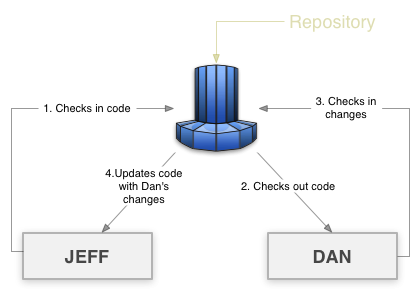
\includegraphics[width=0.8\textwidth]{scm_simple.png}
        \caption{A basic Version Control System}
        \label{sg:fig:scm_simple}
    \end{figure}
\end{frame}

\begin{frame}
    \frametitle{Version Control Workflow}
    \framesubtitle{Distributed}
    \begin{figure}[h]
        \centering
            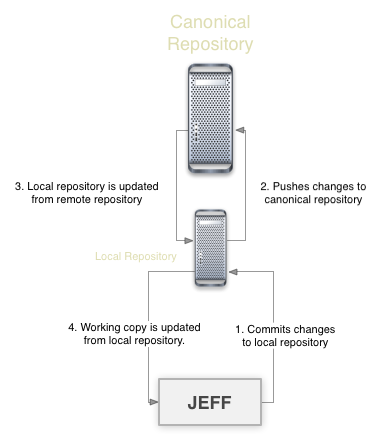
\includegraphics[height=0.8\textheight]{dscm.png}
        \caption{Distributed Version Control System}
        \label{sg:fig:scm_simple}
    \end{figure}
\end{frame}


\begin{frame}
	\frametitle{Why using Version Control}
	\framesubtitle{How it helps}
	
	\begin{enumerate}
		\item<1-> Where do I get the latest (and running) version of a program
		\item<2-> How can we work together on some code, without always sending files, ect..
		\item<3-> I don't understand this code, who wrote that line
		\item<4-> S***, I made some \emph{improvements} and now it does not work anymore 
	\end{enumerate}
	
\end{frame}

\begin{frame}
	\frametitle{Some Guidelines}
	\framesubtitle{that make it easier for everybody}
	\begin{itemize}
		\item<1->commit often
		\item<2->pull often
		\item<3->only running code
		\item<4->code vs. results
		\item<5-> comments
		\item<6-> commit messages
		\item<7-> gitignore 
	\end{itemize}
\end{frame}

\begin{frame}
	\frametitle{Remarks}

	\begin{itemize}
		\item<1-> can be used also with binary data (images, poster, data)
		\item<2-> also local repositories are really useful
		\item<3-> the homework will help you to get some experience
		\item<4-> play with it, it can really help you and the whole lab a lot
		\item<5-> ask me whenever you have questions
	\end{itemize}
		
\end{frame}



\end{document}
